先述のHL7などの共通の規格が活用されていない現実があるので,
いろんな規格の差を吸収できるようなアプリは需要があると考える.
三重県にこのような医療ネットワークを実現するためのたたき台として
本研究では開発を進めた.

\subsection{SQL版について}
 医療大から要望があったエクセル形式のデータについてのアプリは
  Djangoで開発した.

\subsection{SQL版が有する機能}
  \subsubsection{データ入力}
    SQLのテーブルに則った診断データと投薬データの
    CSVファイルであればファイルで入力することができる.

    \begin{figure}[htbp]
  		\begin{center}
  			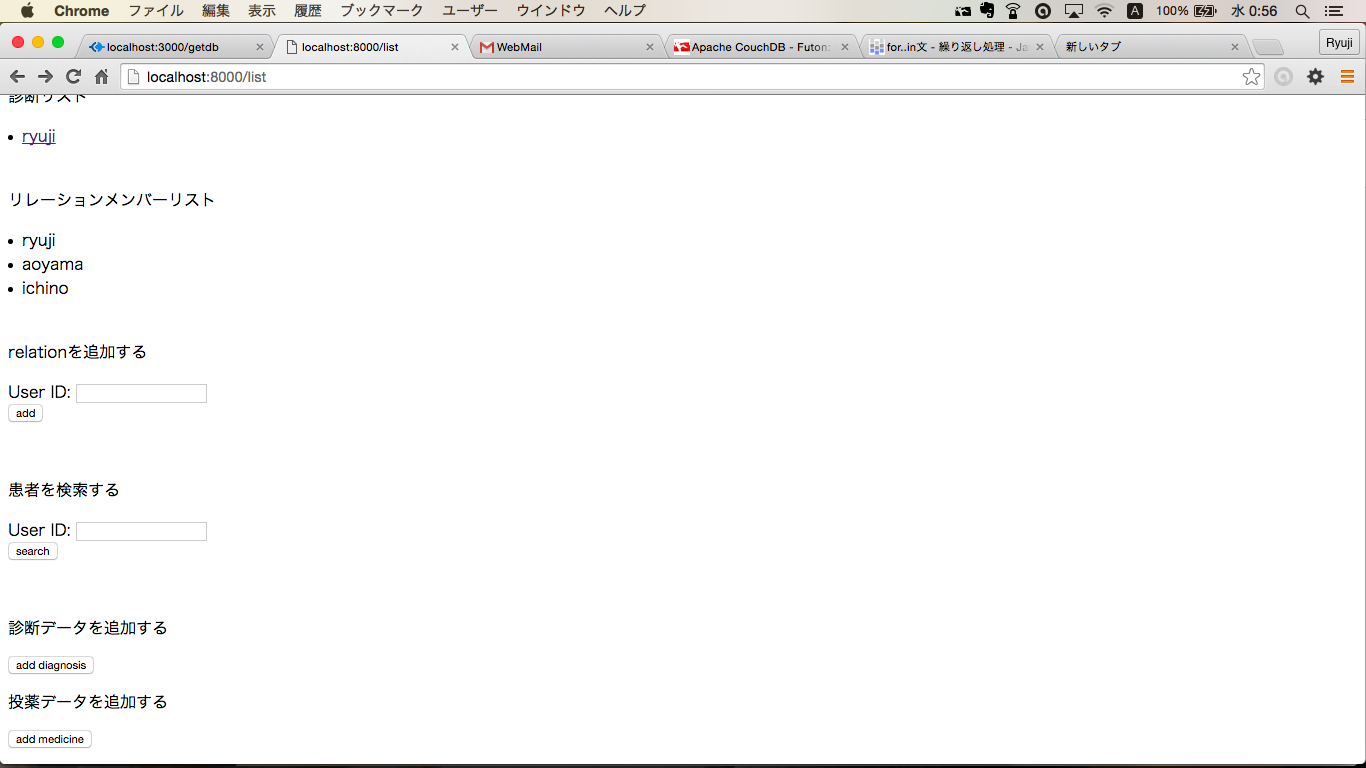
\includegraphics[width=5cm, bb=0 0 645 790]{./gazou/DjangoFileio.png} %よこたて
  		\end{center}
  		\caption{データ入力}
  		\label{DjangoFileio}
  	\end{figure}

  \subsubsection{データ閲覧}
    診断データは表にして、縦方向に診断項目,
    横方向に診断を行った日をとっている.

    \begin{figure}[htbp]
      \begin{center}
        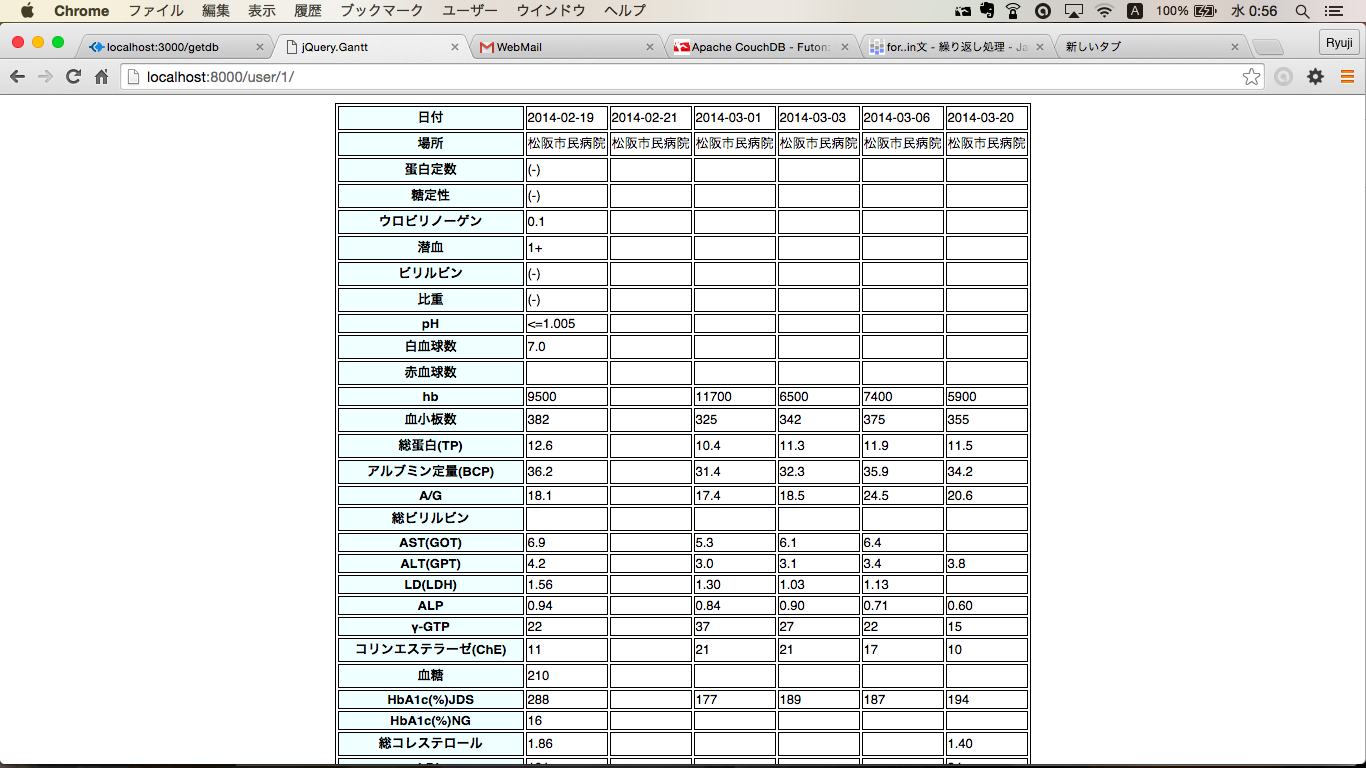
\includegraphics[width=5cm, bb=0 0 645 790]{./gazou/DjangoTable.png} %よこたて
      \end{center}
      \caption{表によるデータ閲覧}
      \label{DjangoTable}
    \end{figure}

    \begin{figure}[htbp]

      投薬データはある薬をどれだけの期間服用しているかを
      わかりやすくするためにガントチャートのように表示している.
      これにより飲み合わせの薬を視覚的に見つけやすくすることができる.

      \begin{center}
        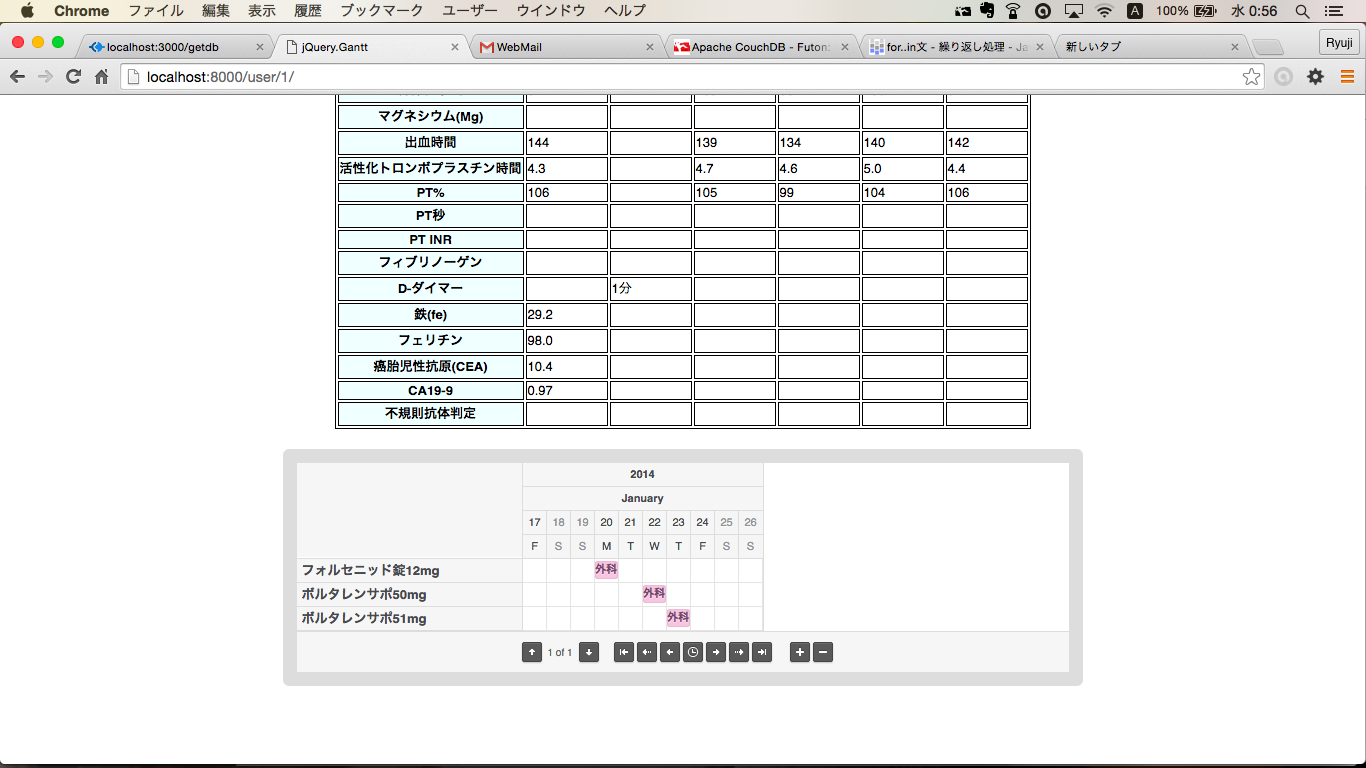
\includegraphics[width=5cm, bb=0 0 645 790]{./gazou/DjangoGantt.png} %よこたて
      \end{center}
      \caption{ガントチャートによるデータ閲覧}
      \label{DjangoGantt}
    \end{figure}

  \subsubsection{権限の付与}
    医療情報を誰が操作することができるかを
    患者が選択する.
    これにより,患者のプライバシーを保護する.


\subsection{SQL版の課題とフィードバック}

  開発アプリのデモンストレーションによって得た医療関係者からの意見の中で
  研究課題として任意の検査項目の抽出が挙げられる.

  他の意見はインターフェース寄りの要望が多かった.
  例えば,表によるデータの表示に対するフィードバックとして,
  任意の検査項目にハイライトをつけてほしいといった内容であったが,
  本研究で工数を割くことができなかったため開発を見送った.


\subsection{NoSQL版の目標設定}
  デモンストレーションから得た課題を解決するには,
  まず入力データの言葉の揺れへの対応が必要となる.
  具体的には,

  今後需要があるであろうバイタルデータの活用に向けて,
  NoSQLを用いたアプリ開発を行う.

  \if0
  ドキュメントの数だけSQLデータベースのテーブルを用意する必要がある.
  データを検索する際にはjoinしてから.
  比べてNoSQLならガンガン入れて,
  データを出すときにだけKeyの関連づけをすればよい.
  NoSQLならSQLに比べてテーブルを用意する分の
  コストがはぶけてる(と言えるかな).
  \fi
